\documentclass[a4paper, 10pt]{article}
\usepackage{geometry}
\geometry{left=3cm,right=3cm,top=3cm,bottom=3cm}
\usepackage{footmisc}
\usepackage[UTF8]{ctex}
\usepackage{amsmath}
\usepackage{subfigure}
\usepackage[graphicx]{realboxes}
\setlength{\parindent}{0pt} 
\begin{document}
\title{{ \textbf {part of reading}}}
  \author{yike}
  \date{}
  
  \maketitle
\section{25.1.15}
\subsection{note of class}
\begin{figure}[ht]
    \centering 
    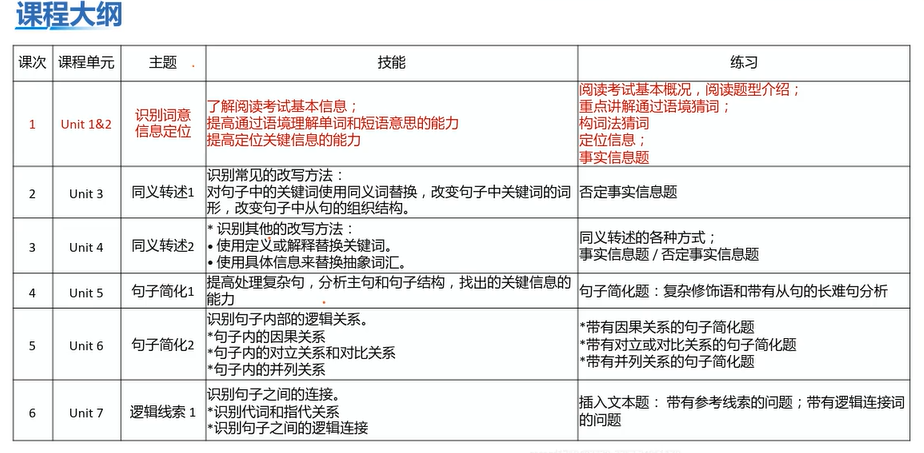
\includegraphics[height=8cm,width=14.5cm]{pic1.png}
    
    
    \label{2}
    
    \end{figure}
types of questions:

1.factual information

2.negative factual information

3.vocabulary

4.reference 指代

5.sentence simplification句子简化

6.inference

7.rhetorical purpose修辞目的

8.insert text句子插入

9.prose summary

36min/2×10q

\subsubsection{some prefixes, suffixes and roots}
\begin{figure}[ht]
    \centering 
    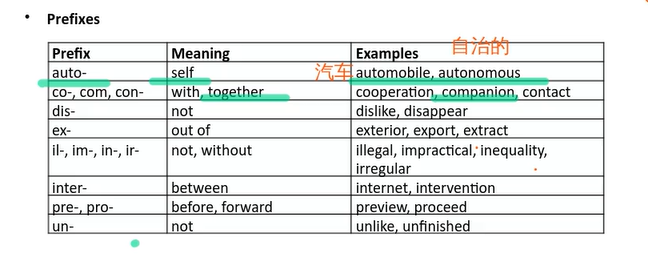
\includegraphics[height=6cm,width=14.5cm]{pic2.png}
    
    
    \label{2}
    
    \end{figure}
    \begin{figure}[ht]
        \centering 
        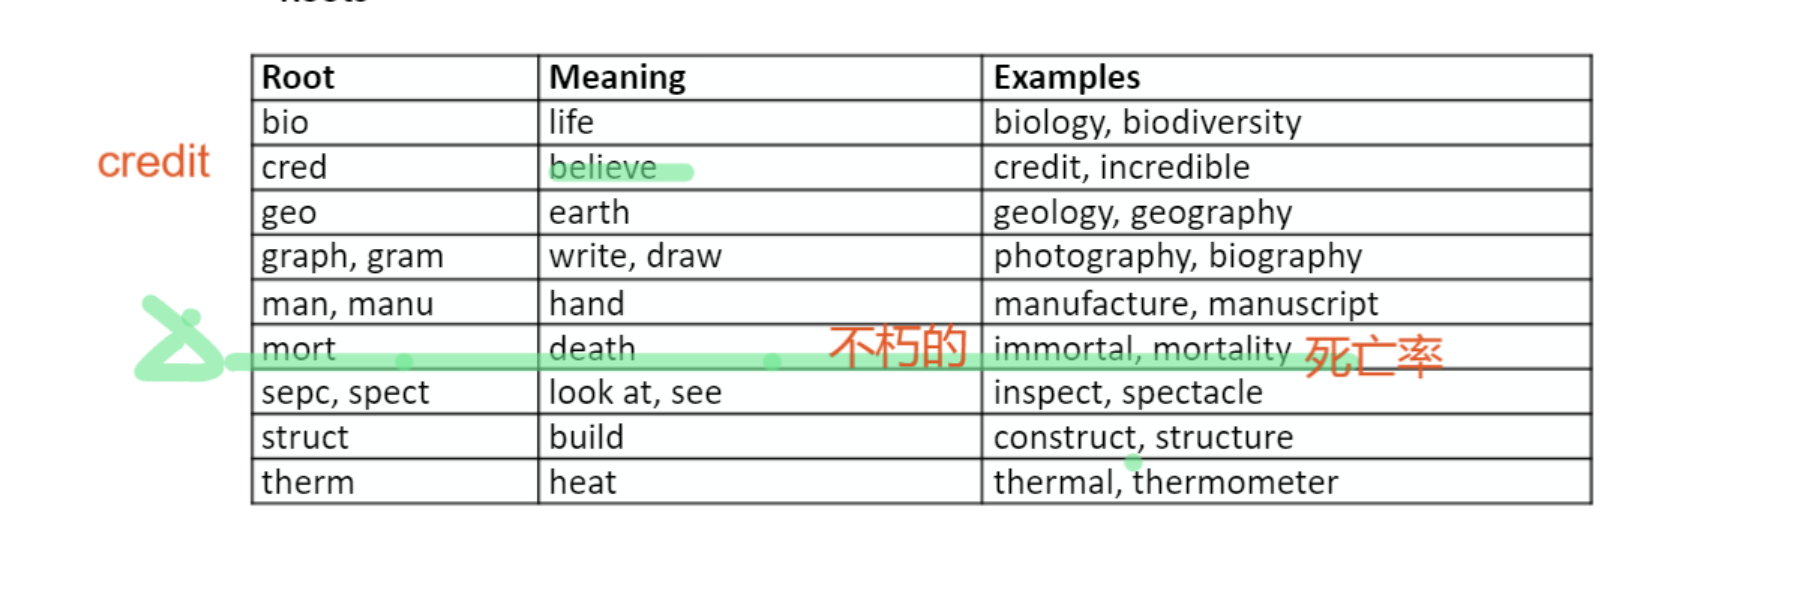
\includegraphics[height=5cm,width=14.5cm]{pic3.png}
        
        
        \label{2}
        
        \end{figure}

        \begin{figure}[ht]
            \centering 
            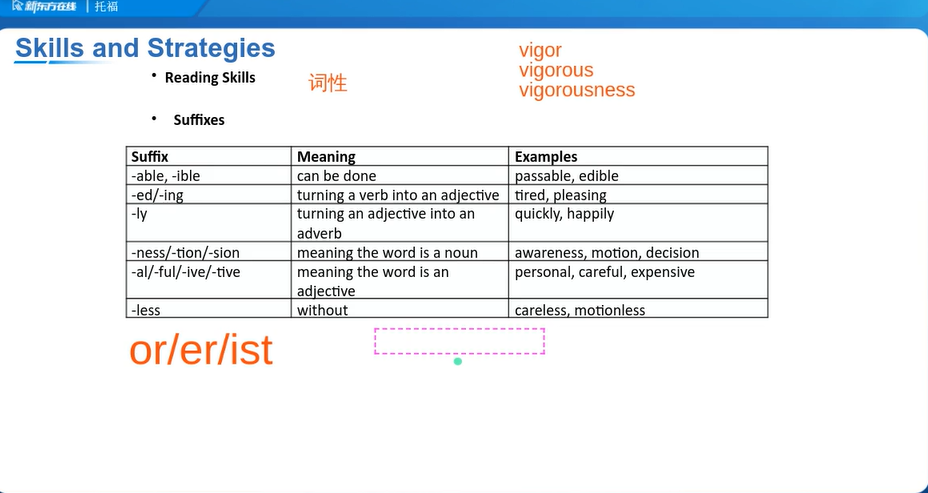
\includegraphics[height=7.5cm,width=14.5cm]{pic4.png}
            
            
            \label{2}
            
            \end{figure}

verb***


生词:orientaion方向、目标n;navigation导航n

难句:the question\textbf{ is not} why they would leave the cold of winter so much\textbf{ as} how they find their way around. 




note:答案不一定一定要包含问题中提到的主语?

still night无风的夜晚

piercing敏锐的,有洞察力的adj;刺穿、突破v;耳洞、洞n

characterize 描述、刻画

densely 密集地,稠密地;难懂地,费解地

vegetation 植物,植被

simultaneously同时地

courtship 求婚,求爱期

ritualized仪式化的

in close quarters近距离接触

vertical垂直的

dispersion传播、分布n

substance物质、主要内容

aggregate总计的adj,集合nv

gravel碎石、沙砾n

cement水泥、胶合剂n

sewer下水道,阴沟;缝纫工,缝纫机

tensile strength抗拉强度

complement补足

endowed with具有,天生具有

compressive压缩的

procurable可得到的、可实现的

thin薄的,细的

mandate授权、委托、命令

recreational娱乐的、消遣的

aqueducts 导水管、沟渠

ballads歌谣

miscellany混合物、混杂

discarded丢弃的、废弃的

devotion挚爱、忠诚、奉献

scatter播撒、散开,零星分布的东西

archaeologists考古学家

patchy零散的,分布不均的、不完整的

precipitation降水、沉淀、轻率、坠落

pottery陶器、陶土、粘土

ally同盟国、盟友、与...结盟

ps1:1.15的生词已经列出,后面一些单词还没来得及查意思,后续会补上。

ps2:今天上课略略有点困没有在课上作系统的笔记,所以晚上整理的时候基本上主要是课上文章的生词,后面会尽量记录上课讲到的思路,不过如果老师能把ppt发到群里会不会比较好?因为拉视频的进度条来翻ppt略微有些麻烦。

\subsection{homework day1}

U1 practise


B  C  D  B  D  C(正选D)  B(正选D)  第八题不太会,正选C


U2 practise

A  D  D  A(正选D)  B

ps:错因分析和作业里的单词积累后续再写吧熬的有点晚.


\subsection{question}
请问课上的那道题,问为什么声音是更好的信息传播方式,我觉得逻辑上的回答应该是“因为声音传播有blabla的好处”,所以选了一个解释声音的选项,但是那道题的正项是解释“因为视觉传播有blabla的缺点”。请问这样是可以的吗?就是它问为什么a是更好的,在选择中我是可以选“因为b有blabla的缺点”这样的选项的吗?感觉有点奇怪。

疑问解答:原文是直接有写sound传播好处的就是几乎不受阻碍,这就是直接原因。这个题选了对比的visual缺点是因为后面的词汇题想强调的是一个前后对比,根据对比关系判断impediment的意思。所以这边这个题是为了后面词汇题服务。

\section{25.1.16}

\subsection{note of class}

topic事实信息题:通常相关信息在一到两个句子中

step1:读题画关键词

step2:定位与关键信息相关的句子

step3:同义转换(topic of today)

关键词:数字、大写字母、限定词(最高级、only等)、时间

constitute

提问方式:关于X的true?/关于X发生的原因?

逻辑词的同义转换:lead to/cause/result in/support/encourage/reflect/derive from/stem from/bring about(引起)/contribute to/attribute to(归因于)...

marsh沼泽

break down拆开,使无效,停止运行

shrimplike像虾的

fiddler小提琴手

snail蜗牛,缓慢移动

decay破败、衰落、腐烂

excrete排泄、分泌

excavation发掘、挖掘、发掘现场

vessel容器、血管

archive档案

审题!!!

irrigation灌溉

ps:感觉区分NG和F似乎不是很有必要,只要知道都是错项就好了

peasant农民

rotation轮作农作物:同一块土地上,根据不同农作物生长的时间来轮流种植

否定事实信息题:except

forage觅食,采集野果

equatorial赤道的

fluidity流动性

specialization专业化 

prestige声望、受尊重的

totemism图腾崇拜

anthropomorphism神人同形同性论

\begin{figure}[ht]
    \centering 
    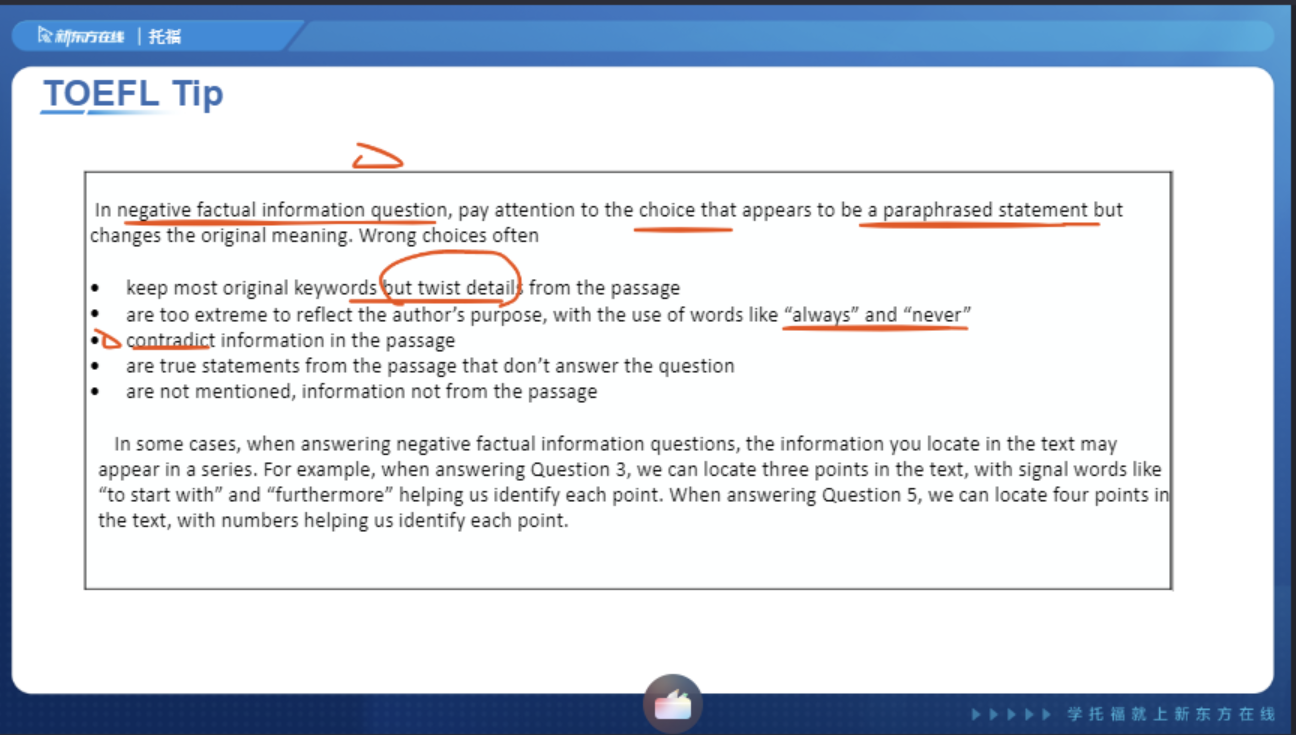
\includegraphics[height=7.5cm,width=14.5cm]{pic7.png}
    
    
    \label{2}
    
\end{figure}

genomes基因组

precede处在...之前

omnivores杂食动物、不偏食的人

tropical热带的


checkerboard棋盘格

prairie草原

fence篱笆

answer all qs except提问方式,选项是一些问题


slushy泥泞的;融雪的;厨子

translocation位置转变

sedentary久坐的

\subsection{homework day2}

D  D(正项C,但我觉得D同样没有提及)  D  D  D

\subsection{question}
我认为这里解析给的这句仍然没有提及到底是火星历史上的哪一时期,所以回答不了D项“during what period”的提问,但答案给的是C,不理解。

\begin{figure}[ht]
    \centering 
    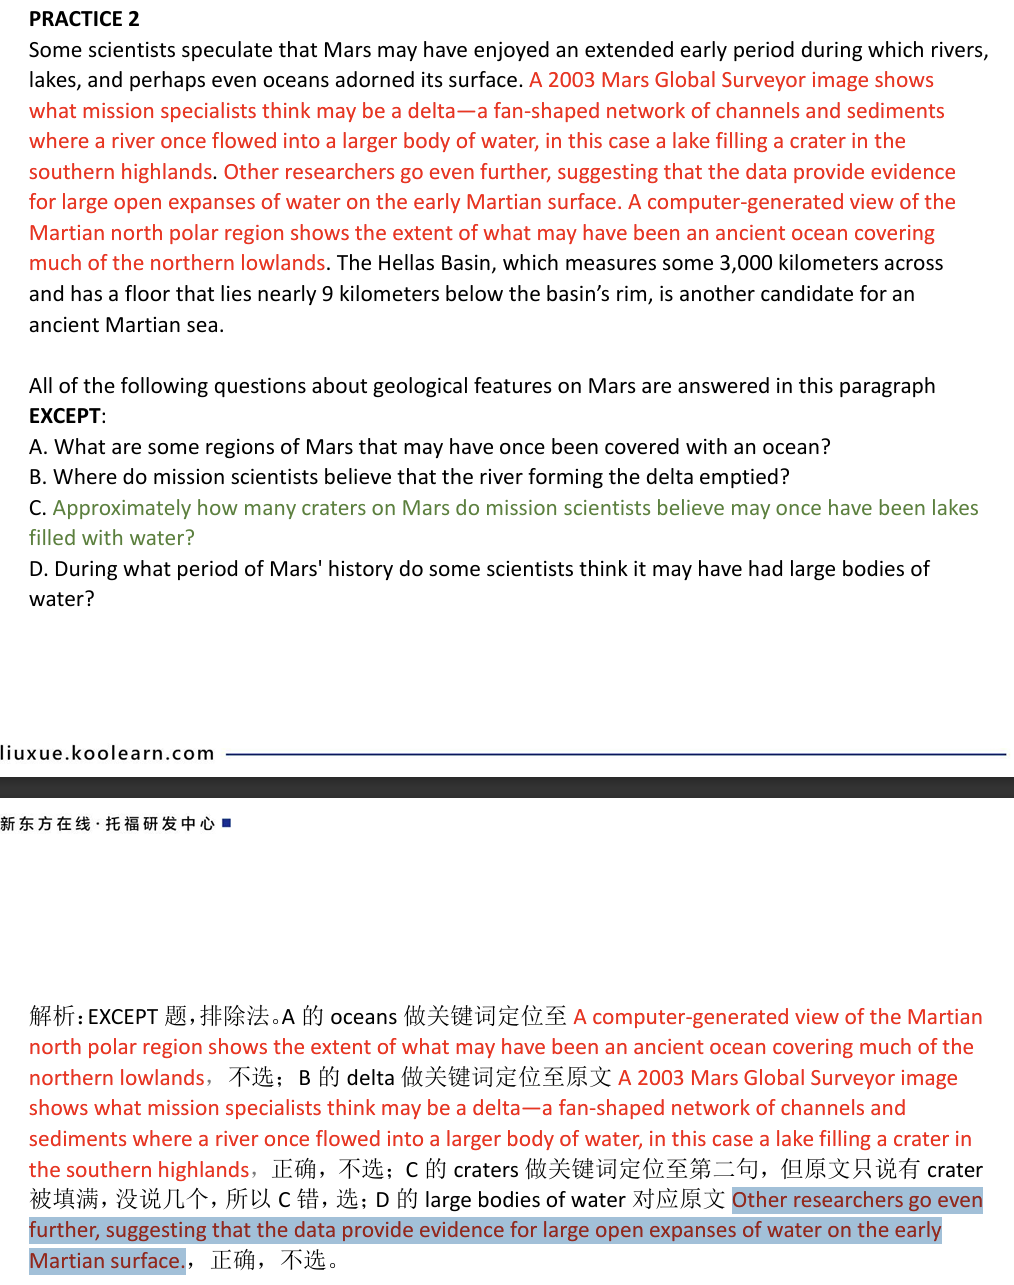
\includegraphics[height=17cm,width=14.5cm]{pic8.png}
    
    
    \label{2}
    
\end{figure}

\section{25.1.17}
\subsection{note of class}

继续同义转述

corruption腐败

lag滞后

protectionist

grandiose过于宏伟的

同义转换:用定义解释一个关键词/用具体信息解释抽象名词/同义词替换

caravans车队

limestone石灰石

key words:问细节的、问因果的

hamlet小村庄

tribal部落的、部族的


herd兽群、人群

sparse植被稀疏的

restock补货

fauna动物

floral植物

\subsection{homework day3}

U4 A  D  B  C  D


\section{25.1.19}

\subsection{note of class}
句子简化题

原文挑一句话,选择与高亮句描述相同意思的选项。

句子主干:谁干了什么事/什么东西是怎么样的

1.识别动词

2.识别主语和宾语

3.修饰宾语

4.系动词 be

5.表语

波折号:插入语,拿掉不影响句子意思

从句:把单词替换成句子

a of b 名词所有格,不拆

frugally节俭地

withered枯萎的

crisp脆的

cached贮藏(cache)

注意逻辑关系,有逻辑关系就要选逻辑关系,无则不选

因果 转折 条件 并列 四个逻辑关系?

\subsection{homework day4}
U5  C(正选A,错误理解了原句的逻辑关系,以为是并列关系)  B  B  D(正选A,词汇量太少以及句子结构没看懂,完全没读懂原句。。。)  C

proliferation激增

innumerable无数


repertoire可表演项目;(某人的)全部才能,全部本领

In the first place, the proliferation of archaeological discoveries and this includes some of the world's innumerable rock art sites that cannot be dated-has served to emphasize a remarkably limited repertoire of subjects.

首先,考古发现的激增,包括世界上无数无法确定年代的岩石艺术遗址,突显了极其有限的主题。

\section{25.1.20}\
\subsection{note of class}
逻辑关系

条件、对比、比较、因果

mutation

divergence

allopatric

speciation

spinescent

thorn

ungulate

palatable


\section{2.4}
\subsection{on class}

反向选择:直接对原文内容取反

topography 地形学

inundation 淹没,水灾

对比取反、时间节点取反

vadose zone渗流层

timber木材/伐木

mutation基因变异

divergence差异

\subsection{homework}

1.BC  2.B  3.A  4.D(正选B,没理解定位句的意思)  5.C






\end{document}

